\chapter{Experimental Evaluation and Controlled DoS Experiment}
\label{chap:experimental-evaluation}

The previous chapters described the framework as a software system: the input
model, the validation rules, the generation of Kathar\'a artefacts, and the
lifecycle used to start and inspect a generated laboratory. This chapter moves
from implementation to experimental use. Its purpose is to verify that the
framework can support a repeatable network experiment in which several
legitimate hosts access the same service concurrently and their observations
are collected before and during a controlled adverse workload.

The experiment is intentionally bounded and is executed entirely inside the
local Kathar\'a environment. No traffic is directed towards external systems.
The adverse workload is therefore used as an experimental condition rather
than as a general-purpose attack mechanism. The objective is to observe how a
finite-capacity TCP application behaves when many connections compete for its
available service slots, and to determine whether client-side and server-side
measurements can describe that transition quantitatively.

\noindent\textbf{Real-world DDoS context.}
The controlled experiment should be interpreted against the broader evolution
of Distributed Denial-of-Service attacks. Real incidents can exhaust different
resources and can rely on compromised botnets, reflection and amplification,
protocol-specific techniques, or application-layer request floods
\cite{rfc4732}. The laboratory developed in this thesis does not attempt to
reproduce the scale, source diversity, or attack infrastructure of such
incidents. Instead, selected cases are useful because they identify several
distinct mechanisms that a small emulated experiment can abstract only in
part.

\begin{table}[htbp]
\centering
\small
\begin{tabular}{p{0.18\textwidth}p{0.32\textwidth}p{0.38\textwidth}}
\toprule
\textbf{Incident} & \textbf{Main characteristic} & \textbf{Relation to this thesis} \\
\midrule
Mirai / Dyn, 2016 &
A Mirai-variant botnet composed of compromised Internet-of-Things devices was
used in DDoS activity that impacted Dyn's DNS infrastructure and disrupted
access to multiple major Internet services \cite{doj_mirai_dyn_2020}. &
This is the closest structural analogy to the controller and multiple load
agents used in the Kathar\'a testbed: several distributed sources converge on
a common service. The laboratory agents, however, are deliberately controlled,
bounded, and non-compromised. \\

GitHub, 2018 &
A memcached UDP reflection/amplification attack reached a peak of
1.35~Tbps and 126.9 million packets per second
\cite{github_ddos_2018}. &
This case illustrates a mechanism that is intentionally not reproduced by the
framework. The attack relied on reflectors, source-address spoofing, and
amplification rather than on direct TCP connection generators. \\

Google HTTP/2 Rapid Reset, 2023 &
A Layer~7 campaign using the HTTP/2 Rapid Reset technique reached a peak of
398 million requests per second. The underlying issue was tracked as
CVE-2023-44487 \cite{google_rapid_reset_2023}. &
The event shows that DDoS intensity cannot be described only in bit/s. Request
rate and server or proxy processing capacity may also become the limiting
resource, which is conceptually closer to the finite application capacity
studied in this chapter. \\

Cloudflare, 2025 &
Cloudflare reported blocking a 7.3~Tbps multi-vector DDoS attack that delivered
37.4~TB in 45 seconds; approximately 99.996\% of the traffic was classified as
UDP floods \cite{cloudflare_ddos_2025}. &
This case illustrates the modern hyper-volumetric and short-duration extreme.
The present experiment deliberately studies a different question: the
relationship between offered workload and available service capacity, rather
than Internet-scale throughput. \\
\bottomrule
\end{tabular}
\caption{Selected real-world DDoS incidents used to contextualise the controlled experiment.}
\label{tab:real-world-ddos-cases}
\end{table}

DDoS is also used outside purely criminal or commercial contexts. Europol's
2026 Internet Organised Crime Threat Assessment describes the pro-Russian
NoName057(16) network as a prominent example of ideologically motivated DDoS
activity. In July 2025, Operation Eastwood disrupted more than 100 servers
associated with the infrastructure; Europol linked the network to an average
of 73 DDoS attacks per day against Ukrainian public and private actors and
reported that activity resumed after an initial decline
\cite{europol_iocta_2026}. This example is relevant because it shows that the
availability objective of a DDoS attack can remain similar even when the
operational motivation and infrastructure are very different.

These cases define an important boundary for the evaluation. The experiment
does not claim to reproduce an Internet-scale botnet, reflection/amplification,
HTTP/2 protocol exploitation, or multi-terabit flooding. Because several
controlled agents contribute simultaneously, the workload has a
distributed-source structure, but the term \emph{controlled DoS} is retained
to emphasise the deliberately bounded laboratory scope. What the experiment
does reproduce is a narrower and measurable resource-contention mechanism:
multiple sources compete with legitimate clients for finite service capacity.
Consequently, the most relevant variables are not absolute traffic volume but
application completion, lower-layer reachability, response time, and the
server-side capacity state. Sections~\ref{sec:measurement-baseline} and
\ref{sec:controlled-dos-results} measure these variables directly.

The archived project contains five complete repetitions for each topology,
collected on 13 October 2026 with the same eight clients, ten concurrent
measurement rounds, and controlled workload schedule. The direct-server runs
are stored under \path{results/dos_lab/simulation_0001/} through
\path{simulation_0005/}; the five complete reverse-proxy runs are stored under
\path{results/mitigation/simulation_0002/} through
\path{simulation_0006/}. Each run contains a baseline and a controlled-load
phase, and every phase file contains 80 client observations. The resulting
dataset therefore comprises 1,600 client observations: 800 per topology and,
within each topology, 400 for the baseline and 400 for the controlled-load
phase. The final dataset was defined as executions containing both client-phase
CSV files with 80 observations per phase together with the server-side metric
files; no observation from a run satisfying this completeness criterion was
excluded. The directory \path{results/mitigation/simulation_0001/} is a
preliminary pilot collected before the routing-readiness criterion was added.
It contains server metrics but no client-result CSV and was therefore never a
member of the final dataset. The first complete run of each topology is
retained below as a detailed representative execution;
Section~\ref{sec:repeated-run-validation} then treats the ten complete runs as
the descriptive dataset. All numerical results were recalculated directly from
the archived CSV files rather than transcribed from console output.

\section{Experimental Methodology and Testbed}
\label{sec:experimental-methodology}

The experimental testbed is generated from \path{configs/dos_lab.yml}. It is a
multi-LAN enterprise-style topology composed of two legitimate-user networks,
a routed core, a separate network containing the controlled load agents, and a
DMZ containing the application server. All routers use OSPF in area 0, so the
experiment also depends on the routing configuration produced by the framework
rather than on a single flat collision domain.

The two legitimate LANs contain four hosts each. The first LAN uses the
prefix \texttt{10.10.1.0/24} and contains \texttt{pc\_a1} through
\texttt{pc\_a4}; the second uses \texttt{10.10.2.0/24} and contains
\texttt{pc\_b1} through \texttt{pc\_b4}. The target service is hosted by
\texttt{server} at \texttt{10.30.1.10/24} in the DMZ. A separate workload
network uses \texttt{10.20.1.0/24} and contains the controller
\texttt{attacker} together with three bounded load agents,
\texttt{zombie\_1}, \texttt{zombie\_2}, and \texttt{zombie\_3}. The
corresponding collision-domain names are reported in the configuration and the
functional roles are summarised in Table~\ref{tab:experimental-nodes}.

\begin{table}[htbp]
\centering
\small
\begin{tabular}{p{0.24\textwidth}p{0.28\textwidth}p{0.36\textwidth}}
\toprule
\textbf{Component} & \textbf{Nodes / address range} & \textbf{Role} \\
\midrule
Legitimate LAN A & \texttt{pc\_a1}--\texttt{pc\_a4}, \texttt{10.10.1.0/24} & Concurrent legitimate clients connected through \texttt{r1}. \\
Legitimate LAN B & \texttt{pc\_b1}--\texttt{pc\_b4}, \texttt{10.10.2.0/24} & Concurrent legitimate clients connected through \texttt{r2}. \\
Routing core & \texttt{r1}, \texttt{r2}, \texttt{r3}, \texttt{r4}, \texttt{core} & OSPF infrastructure connecting the client LANs, the DMZ, and the isolated workload LAN. \\
Service DMZ & \texttt{server}, \texttt{10.30.1.10/24} & Instrumented TCP application exposed on port \texttt{9000}. \\
Controlled-load LAN & \texttt{attacker}, \texttt{zombie\_1}--\texttt{zombie\_3}, \texttt{10.20.1.0/24} & Controller and bounded connection generators used only inside the laboratory. \\
\bottomrule
\end{tabular}
\caption{Main components of the experimental topology.}
\label{tab:experimental-nodes}
\end{table}

Figure~\ref{fig:dos-testbed} shows the logical structure of the testbed. The
central point is that legitimate traffic and controlled workload traffic reach
the same server through the routed infrastructure. This makes the experiment a
test not only of the application but also of the complete laboratory generated
by the framework: addressing, gateways, inter-router links, OSPF routes, node
resources, and service startup commands all have to operate consistently.

\begin{figure}[htbp]
\centering
\resizebox{0.94\textwidth}{!}{%
\begin{tikzpicture}[
    node distance=10mm and 14mm,
    host/.style={draw, rounded corners, align=center, minimum width=2.3cm, minimum height=8mm},
    router/.style={draw, diamond, aspect=2.1, align=center, inner sep=1.2pt},
    net/.style={draw, dashed, rounded corners, align=center, minimum width=2.6cm, minimum height=8mm},
    line/.style={thick}
]
\node[host] (lana) {4 clients\\LAN A};
\node[router, right=of lana] (r1) {r1};
\node[router, right=18mm of r1] (r3) {r3};
\node[router, below=15mm of r1] (r2) {r2};
\node[router, right=18mm of r2] (r4) {r4};
\node[router, right=18mm of r3, yshift=-10mm] (core) {core};
\node[host, left=of r2] (lanb) {4 clients\\LAN B};
\node[host, right=20mm of core, yshift=11mm] (server) {server\\10.30.1.10};
\node[host, right=20mm of core, yshift=-14mm] (load) {attacker +\\3 agents};

\draw[line] (lana) -- node[above]{\scriptsize \texttt{lan\_a}} (r1);
\draw[line] (lanb) -- node[below]{\scriptsize \texttt{lan\_b}} (r2);
\draw[line] (r1) -- (r2);
\draw[line] (r1) -- (r3);
\draw[line] (r2) -- (r4);
\draw[line] (r3) -- (r4);
\draw[line] (r2) -- (core);
\draw[line] (r3) -- (core);
\draw[line] (r4) -- (core);
\draw[line] (core) -- node[above,sloped]{\scriptsize DMZ} (server);
\draw[line] (core) -- node[below,sloped]{\scriptsize workload LAN} (load);
\end{tikzpicture}%
}
\caption{Logical structure of the controlled experimental testbed.}
\label{fig:dos-testbed}
\end{figure}

The experiment is orchestrated by \path{simulate.sh}. By default the script
selects \texttt{dos\_lab}, targets the node named \texttt{server} on TCP port
\texttt{9000}, discovers all nodes whose names begin with \texttt{pc\_} as
legitimate clients, and creates a new numbered output directory under
\path{results/dos_lab/}. Earlier connectivity utilities were more dependent on
literal addresses; accepting a logical target name where possible reduced the
need to repeat addressing information already represented by the laboratory
configuration and made the same test workflow easier to reuse after address
changes. A full run first performs the baseline measurement and then performs
the controlled-load measurement using the same laboratory and the same
measurement parameters.

The default parameters used by all archived complete runs are ten
simultaneous rounds, a three-second measurement timeout, one second between
rounds, and a 25-second startup wait when the orchestrator starts the lab. The
script also checks reachability of the target from every legitimate client
before starting the measurements. This routing-readiness stage repeatedly sends
an ICMP probe from each client and allows up to 120 seconds for the routes to
become usable. The check was introduced after earlier executions showed that a
measurement could start while dynamic routing was not yet usable from every
client. A fixed startup delay alone was therefore not considered a sufficient
readiness criterion. By checking the observed network state, an OSPF
convergence problem can be detected before it contaminates the service
baseline. This is particularly relevant in light of the preliminary
\path{mitigation/simulation_0001} pilot described above: because it predates
this criterion and contains no client-result dataset, it is retained only as a
development artefact and is not analysed as an experimental run.

Table~\ref{tab:experimental-environment} records the software and host
environment used for the archived experiments. These values were captured on
the experimental host when the results were archived on 13 October 2026. The
Git working tree contained uncommitted changes, so the base commit alone is not
a byte-for-byte identifier of the executed source; the archived project files,
configuration files, raw CSV data, and container-image digests are therefore
the authoritative experimental artefacts.

\begin{table}[htbp]
\centering
\small
\begin{tabular}{p{0.28\textwidth}p{0.62\textwidth}}
\toprule
\textbf{Component} & \textbf{Recorded value} \\
\midrule
Host processor & 11th Gen Intel Core i7-11800H at 2.30 GHz; 16 logical CPUs \\
Host memory & 15 GiB RAM; 2 GiB swap \\
Operating system & Linux Mint 22.2; Linux kernel \texttt{7.0.0-34-generic} \\
Python / PyYAML & Python 3.12.3; PyYAML 6.0.1 \\
Docker & Client and server 29.8.1 \\
Kathar\'a & Version 3.8.3 \\
\texttt{kathara/base:latest} &
\texttt{sha256:8a2e70ac8f51bb283b8549fd686f65f9}\allowbreak
\texttt{a1ef4487fe2c81849cb74d301e61970b} \\
\texttt{kathara/frr:latest} &
\texttt{sha256:3b7a3f630d8ecd9efddd4586ba2f0a41}\allowbreak
\texttt{e2c462f13bc81dee8e3c6ebac183f57c} \\
Framework source & Git base commit \texttt{3a1d65189981}; working tree dirty \\
\bottomrule
\end{tabular}
\caption{Host, software, and container-image metadata recorded for the
experimental archive.}
\label{tab:experimental-environment}
\end{table}

The results of each run are isolated by a run number. Client
measurements are separated by scenario in
\path{connection_results_baseline.csv} and
\path{connection_results_dos.csv}; service-side counters are stored in
\path{server_metrics.csv}; and host-level Docker samples are stored in
\path{server_container_metrics.csv}. The same run identifier is also
used by the logging hierarchy, which makes it possible to associate a client
failure with the corresponding server state and orchestration run. The
mitigation runs retain the same schema: the \texttt{target\_input} field changes
from \texttt{server} to \texttt{proxy}, while the public address and port remain
\texttt{10.30.1.10:9000}.

\section{Measurement Infrastructure and Baseline Evaluation}
\label{sec:measurement-baseline}

The target application is implemented by \path{configs/server/service.py}. It
is a multithreaded TCP service that listens on port \texttt{9000}. A bounded
semaphore, implemented with
\texttt{threading.}\allowbreak\texttt{BoundedSemaphore}, limits the number of
active application sessions. In the experimental YAML and in the orchestration
fallback command, \texttt{SERVICE\_MAX\_ACTIVE} is set to 20 and
\texttt{SERVICE\_BACKLOG} is set to 20. A connection that cannot acquire an
application slot is answered with \texttt{BUSY} when possible and then closed.
A connection that obtains a slot receives a small text menu; selection
\texttt{1} returns the token \texttt{pong}.

This behaviour allows the experiment to distinguish network reachability, TCP
connectivity, and application availability. This distinction grew out of a
concrete development problem: a client could reach the server node while the
application process was not running or was unable to complete the expected
transaction. Treating reachability as a successful service test therefore
produced misleading results. A successful ICMP reply proves only that the
routed path is currently reachable, while a successful TCP handshake proves
that the kernel accepted a connection to the server port. Neither event alone
proves that the application completed the requested operation. For this reason,
\path{run_connection_tests.py} treats a request as successful only when the
client sends \texttt{1} and subsequently observes \texttt{pong} in the server
response.

Each measurement is executed inside the client container rather than on the
Docker host. The script records five timing fields, listed in
Table~\ref{tab:measurement-metrics}. This separation is important because the
host-side time required to invoke \texttt{docker exec} is not a network delay
and should not be interpreted as one.

\begin{table}[htbp]
\centering
\small
\begin{tabular}{p{0.31\textwidth}p{0.57\textwidth}}
\toprule
\textbf{Metric} & \textbf{Meaning} \\
\midrule
\texttt{icmp\_rtt\_ms} & Round-trip time of a single ICMP echo request executed in the client network namespace. \\
\texttt{tcp\_connect\_ms} & Time from the beginning of \texttt{connect()} to successful establishment of the TCP connection. \\
\texttt{application\_response\_ms} & Time between sending selection \texttt{1} and receiving a response containing \texttt{pong}. \\
\texttt{request\_completion\_ms} & Complete TCP application transaction from the start of connection establishment to reception of \texttt{pong}. \\
\path{host_command_completion_ms} & Host-observed duration of the complete measurement command, including Docker invocation overhead. \\
\bottomrule
\end{tabular}
\caption{Client-side metrics recorded by \texttt{run\_connection\_tests.py}.}
\label{tab:measurement-metrics}
\end{table}

The execution model was also changed during development. A sequential strategy
is sufficient when the question is simply whether each client can reach a
service, but it becomes problematic when clients are intended to observe a
shared and time-varying server condition. Executing all attempts from one host
before moving to the next would compare measurements collected in different
windows and could make an overload transition appear different for each client.
For every request index, the final implementation therefore schedules the eight
legitimate clients concurrently through a \texttt{ThreadPoolExecutor}. The
execution model is round based rather than client based: in round~1 all eight
clients perform one measurement; after the configured delay, round~2 repeats
the same operation, and so on. With eight clients and ten attempts, each
scenario produces 80 application requests. Concurrency is therefore an
experimental requirement for comparability, not merely a performance
optimisation.

Application availability is defined as

\begin{equation}
A = \frac{N_{\mathrm{pong}}}{N_{\mathrm{requests}}} \times 100,
\label{eq:application-availability}
\end{equation}

where $N_{\mathrm{pong}}$ is the number of requests for which the expected
application response was received. Failed requests remain part of the
denominator. Latency summaries, on the other hand, can only be calculated from
requests for which the corresponding timing value exists. This distinction is
essential under overload: a low mean response time among the small subset of
successful requests does not imply a healthy service when most requests fail.

As a representative execution, the baseline of
\path{dos_lab/simulation_0001} contains 80 requests and all 80
completed successfully, corresponding to 100\% application availability. All
ICMP probes and all TCP connection attempts were also successful. The mean
ICMP RTT was 1.686 ms and the mean TCP connection time was 1.803 ms. Among the
successful application requests, the mean response time was 3.218 ms, the
median was 3.202 ms, the 95th percentile was 4.922 ms, and the maximum was
5.309 ms. Table~\ref{tab:baseline-summary} reports the main values.

\begin{table}[htbp]
\centering
\small
\begin{tabular}{lr}
\toprule
\textbf{Baseline metric} & \textbf{Value} \\
\midrule
Legitimate application requests & 80 \\
Successful application requests & 80 \\
Application availability & 100.00\% \\
ICMP successes & 80 / 80 \\
TCP connection successes & 80 / 80 \\
Mean ICMP RTT & 1.686 ms \\
Mean TCP connection time & 1.803 ms \\
Mean application response time & 3.218 ms \\
Median application response time & 3.202 ms \\
95th percentile application response time & 4.922 ms \\
Maximum application response time & 5.309 ms \\
Approximate measurement duration & 10.77 s \\
\bottomrule
\end{tabular}
\caption{Direct-server baseline results from \texttt{dos\_lab/simulation\_0001}.}
\label{tab:baseline-summary}
\end{table}

Figure~\ref{fig:direct-baseline-metrics} reports the corresponding per-client
measurements. The availability panel remains at 100\% in every round, while the
other panels show the short-timescale variation in ICMP, TCP, and application
response times summarised in Table~\ref{tab:baseline-summary}.

\begin{figure}[p]
\centering
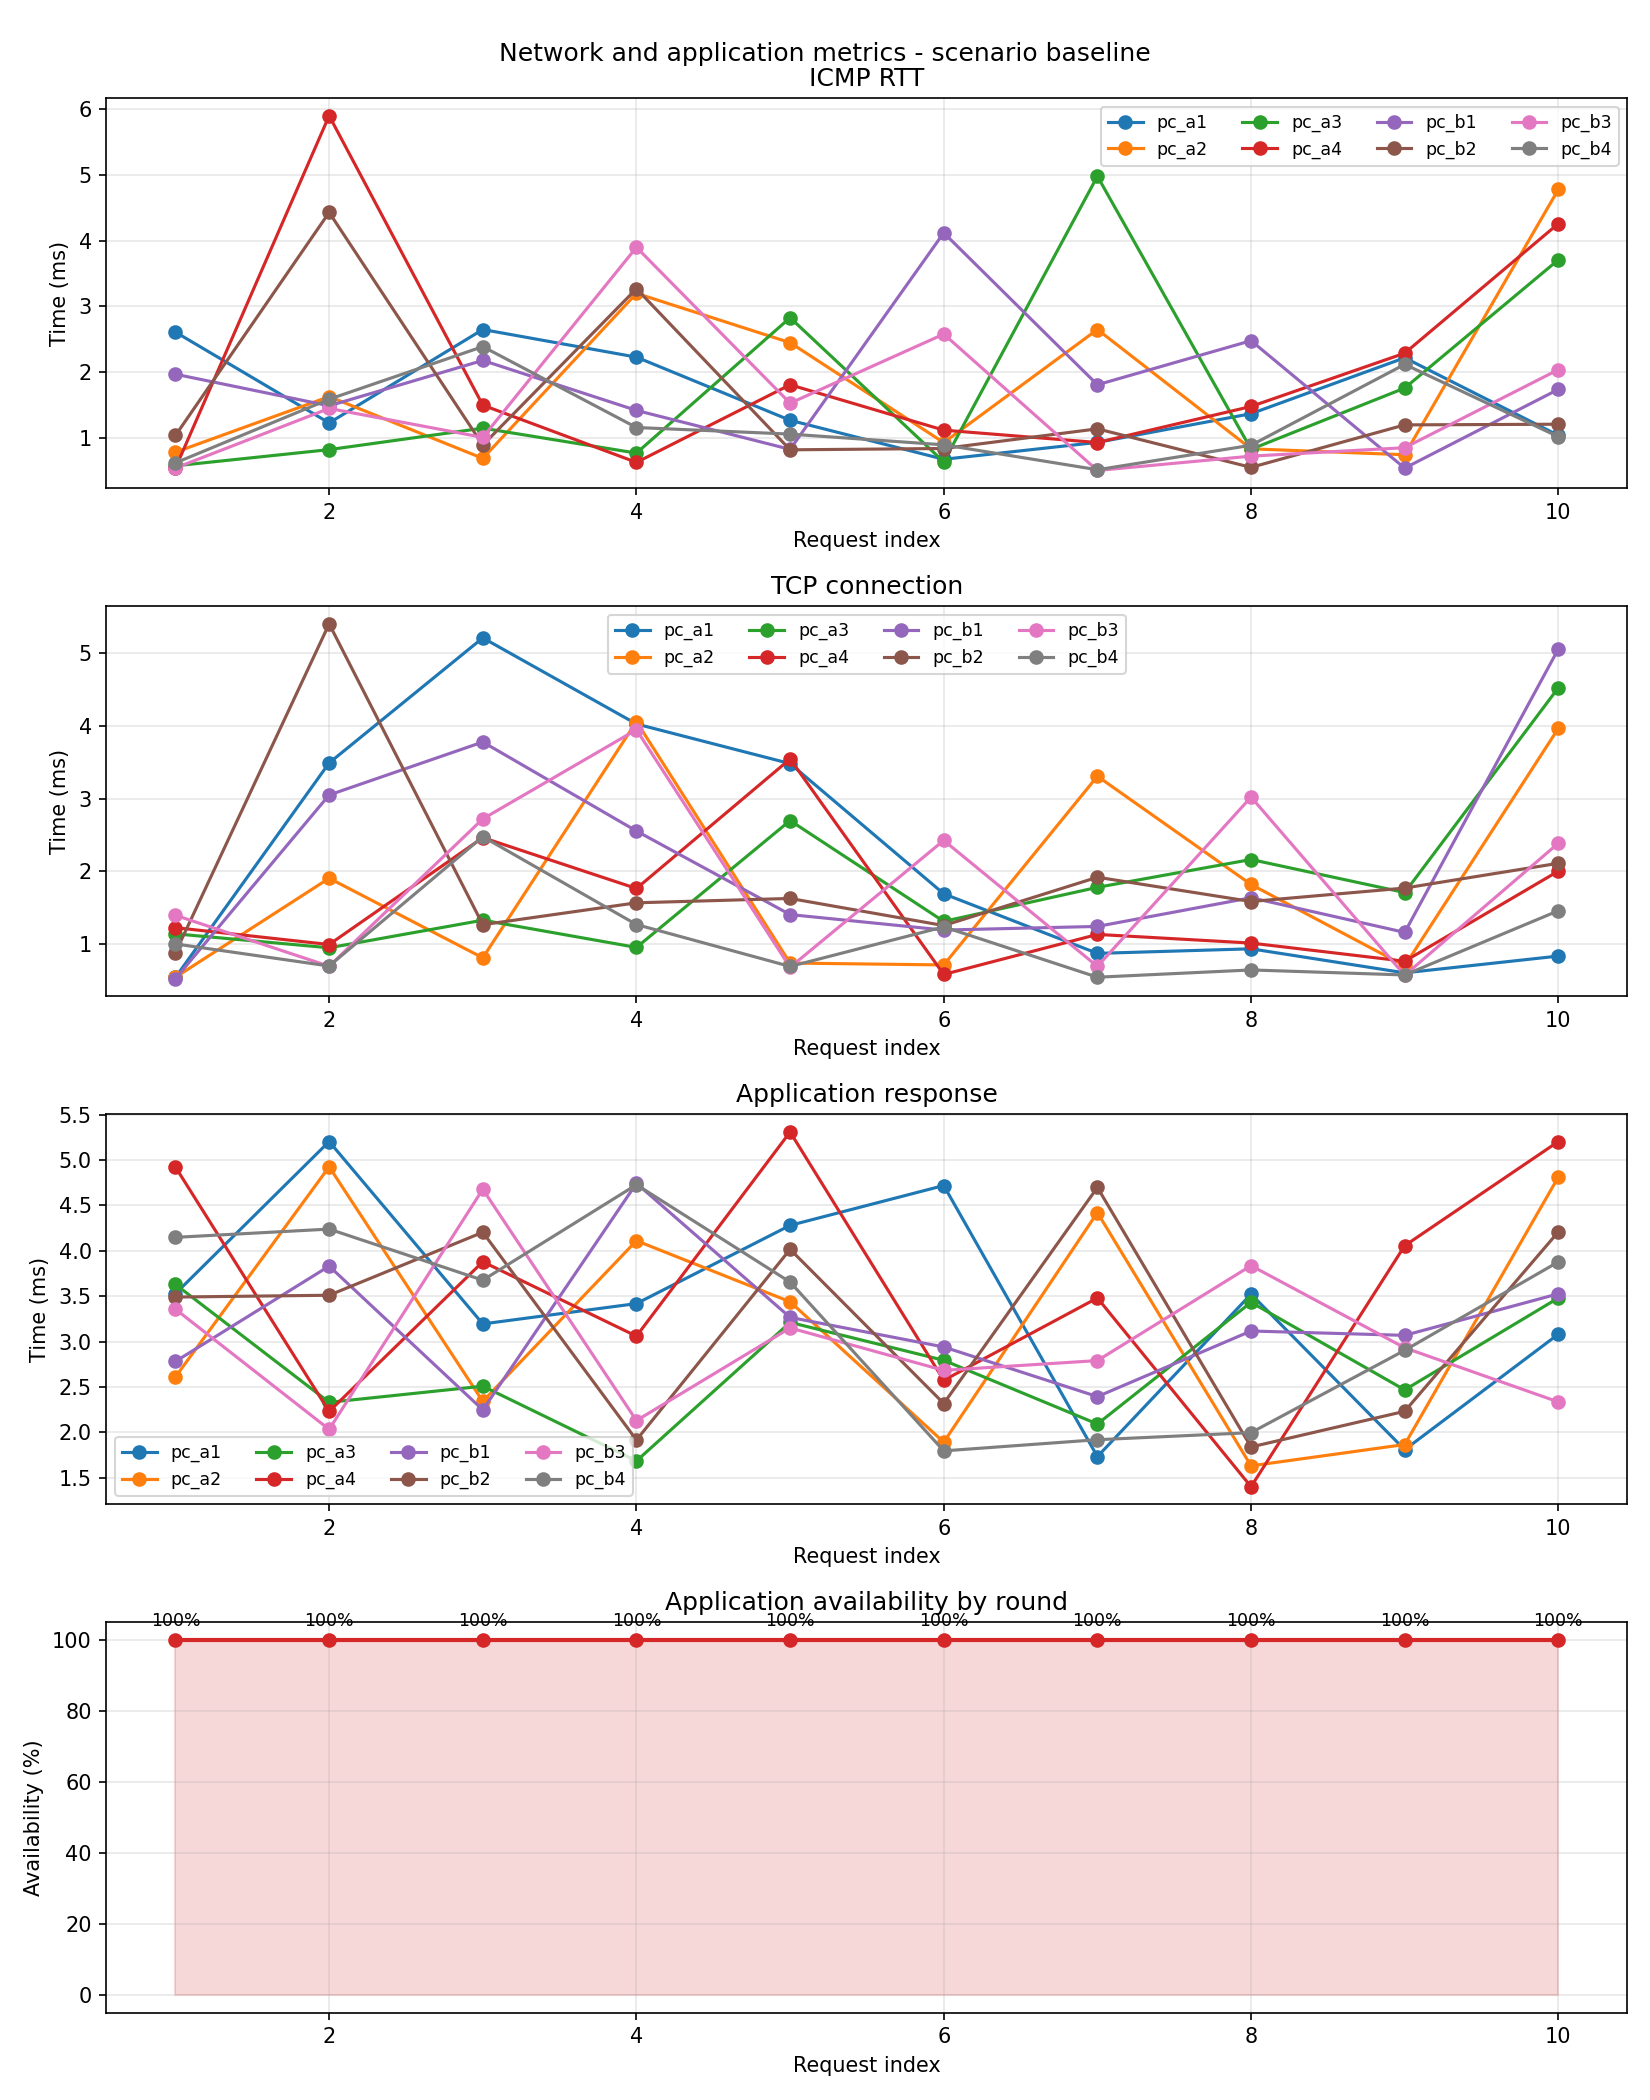
\includegraphics[width=0.90\textwidth]{images/dos_lab_simulation_0001_baseline_metrics.png}
\caption{Per-client network and application measurements for the direct-server baseline in \texttt{dos\_lab/simulation\_0001}.}
\label{fig:direct-baseline-metrics}
\end{figure}

The per-client baseline is also uniform. Every client completed ten out of ten
requests successfully. No client exhibits an availability disadvantage. This
is relevant because the clients are attached
to two different access LANs and traverse different first-hop routers; the
baseline therefore establishes that the generated routing topology does not
itself introduce a visible service failure before the adverse workload is
introduced.

The server-side metrics reinforce the same conclusion. During the baseline
window, the instrumented service recorded 80 accepted connection events and no
\texttt{BUSY} or rejected events. The maximum number of simultaneously active
connections observed by the server was one and the maximum active thread count
was four. The container sampler collected six Docker-stat samples for the
baseline window; these samples reported a mean CPU utilisation of approximately
0.53\% and a maximum of 0.88\%. Since the baseline measurement lasts only about
ten seconds and the container dataset contains a small number of samples, these
resource figures are used descriptively rather than as statistically stable
estimates of host consumption.

The mitigation baseline in \path{mitigation/simulation_0002} independently
satisfies the same validity criteria: all eight clients are present in every
round, all 80 ICMP and TCP checks succeed, and all 80 application transactions
complete. Its application response is slower because the transaction traverses
the proxy: the mean is 6.058 ms, compared with 3.218 ms for the direct-server
baseline. This baseline cost is considered together with the protection result
in Section~\ref{sec:mitigation-results}.

\section{Controlled DoS Experiment and Observed Results}
\label{sec:controlled-dos-results}

The controlled DoS phase was not part of the initial topology-generation
requirement. It was introduced only after generation, routing, and service
measurement were sufficiently stable to support a controlled comparison between
two operating conditions. Reusing the same topology and measurement path was
preferred to building a separate attack-specific environment, because it keeps
the baseline and adverse phases comparable and turns the experiment into an
extension of the existing verification workflow.

The second phase introduces a bounded connection-based workload while the same
eight legitimate clients continue to use the same application interface. The
experiment is best interpreted as connection-capacity contention rather than as
a bandwidth-flooding benchmark. Each controlled agent opens several TCP
connections to the service and attempts to keep them established for a bounded
period. The target application, by contrast, exposes only 20 concurrent
application slots. The expected effect is therefore contention for finite
server-side session capacity, not saturation of a physical link.

The control architecture consists of one \texttt{attacker} node and three
agents. Each agent listens on TCP port \texttt{9999}. The controller reads the
agent addresses from \path{zombies.txt} and sends a command containing the
target address, target port, requested number of connections, and duration. The
orchestrator uses 40 requested connections per agent and a 60-second duration
by default, with an additional global cap that prevents a configured duration
above 90 seconds. With three agents, the requested workload therefore consists
of up to 120 concurrent connection workers competing with a service configured
for 20 active application sessions.

The agents are themselves bounded. The implementation limits the number of
connections created by one agent and limits the duration of a load episode.
Each worker reconnects when necessary so that pressure can be maintained across
the configured interval even if a server-side timeout closes an idle
connection. These restrictions make the mechanism suitable for a repeatable
laboratory experiment: load intensity and duration are explicit parameters and
the agent remains confined to the addresses provided by the controller inside
the generated topology.

The full orchestration does not simply start the workload and then begin
measuring. Client measurement starts first, while workload activation is
scheduled asynchronously after the configured start delay. In the direct-server
run this creates a visible transition within the same result file. The
first two request rounds complete successfully for all eight legitimate
clients; from round 3 onward, none of the legitimate requests receives a valid
\texttt{pong}. Table~\ref{tab:availability-rounds} shows this progression.

\begin{table}[htbp]
\centering
\small
\begin{tabular}{cccc}
\toprule
\textbf{Round} & \textbf{Requests} & \textbf{Successful} & \textbf{Availability} \\
\midrule
1 & 8 & 8 & 100\% \\
2 & 8 & 8 & 100\% \\
3 & 8 & 0 & 0\% \\
4 & 8 & 0 & 0\% \\
5 & 8 & 0 & 0\% \\
6 & 8 & 0 & 0\% \\
7 & 8 & 0 & 0\% \\
8 & 8 & 0 & 0\% \\
9 & 8 & 0 & 0\% \\
10 & 8 & 0 & 0\% \\
\bottomrule
\end{tabular}
\caption{Application availability by request round during the direct-server controlled-load measurement.}
\label{tab:availability-rounds}
\end{table}

Across the complete controlled-load measurement, 16 of 80 legitimate requests
succeeded, giving an overall availability of 20\%. This percentage includes the
first two rounds, which completed before the controlled workload became active.
During the attack-active interval, from rounds 3 through 10, none of the 64
legitimate application requests completed successfully; application
availability while the workload was active was therefore 0\%. The 20\% value
must consequently be interpreted as the availability of the complete transition
run, whereas 0\% describes the period in which the adverse workload was
actually active. Importantly, all 80 ICMP probes succeeded and all 80 TCP
handshakes were recorded as successful. Of the 64 application failures, 47 did
not receive the expected \texttt{pong} and 17 reported a connection reset as
\texttt{socket\_error:104} after the TCP connection had already been
established. The experiment therefore exhibits a
clear separation between network-level reachability and application-level
availability.

This result is one of the central observations of the evaluation. If the test
had relied on \texttt{ping} alone, the service would have appeared fully
reachable during the entire workload window. If it had relied only on TCP
connection establishment, the same conclusion would have been reached, because
all handshakes succeeded. Only the application-level request identifies that 64
of the 80 legitimate transactions did not complete successfully. In other
words, a reachable host and an open TCP port do not imply that the service is
currently able to satisfy legitimate work.

The timing values show the same distinction. Mean ICMP RTT increased from
1.686 ms in the baseline to 2.127 ms during the controlled-load run. Mean TCP
connection time increased from 1.803 ms to 2.198 ms. Among the 16 requests that
still succeeded, mean application response time was 3.432 ms, the median was
3.347 ms, the 95th percentile was 4.567 ms, and the maximum was 4.735 ms.
These successful-request
latencies alone would suggest only modest change. The major degradation is
therefore represented by the fall in completion probability, not by a large
increase in the latency of transactions that happen to complete.

\begin{table}[htbp]
\centering
\small
\begin{tabular}{lrr}
\toprule
\textbf{Metric} & \textbf{Baseline} & \textbf{Controlled run} \\
\midrule
Legitimate requests & 80 & 80 \\
Successful application requests & 80 & 16 \\
Overall application availability & 100.00\% & 20.00\% \\
Attack-active application availability & -- & 0.00\% \\
Successful ICMP probes & 80 & 80 \\
Successful TCP handshakes & 80 & 80 \\
Mean ICMP RTT & 1.686 ms & 2.127 ms \\
Mean TCP connection time & 1.803 ms & 2.198 ms \\
Mean application response time$^{*}$ & 3.218 ms & 3.432 ms \\
Median application response time$^{*}$ & 3.202 ms & 3.347 ms \\
95th percentile application response$^{*}$ & 4.922 ms & 4.567 ms \\
Maximum application response time$^{*}$ & 5.309 ms & 4.735 ms \\
\bottomrule
\end{tabular}
\caption{Client-side comparison for \texttt{dos\_lab/simulation\_0001}. Values marked with $^{*}$ are calculated only from requests that produced an application response.}
\label{tab:client-comparison}
\end{table}

The transition is visible directly in
Figure~\ref{fig:direct-dos-metrics}: application availability is 100\% in the
first two rounds and falls to 0\% from round 3 onward. Application-response
curves consequently stop after round 2, although the ICMP and TCP panels retain
measurements for all ten rounds.

\begin{figure}[p]
\centering
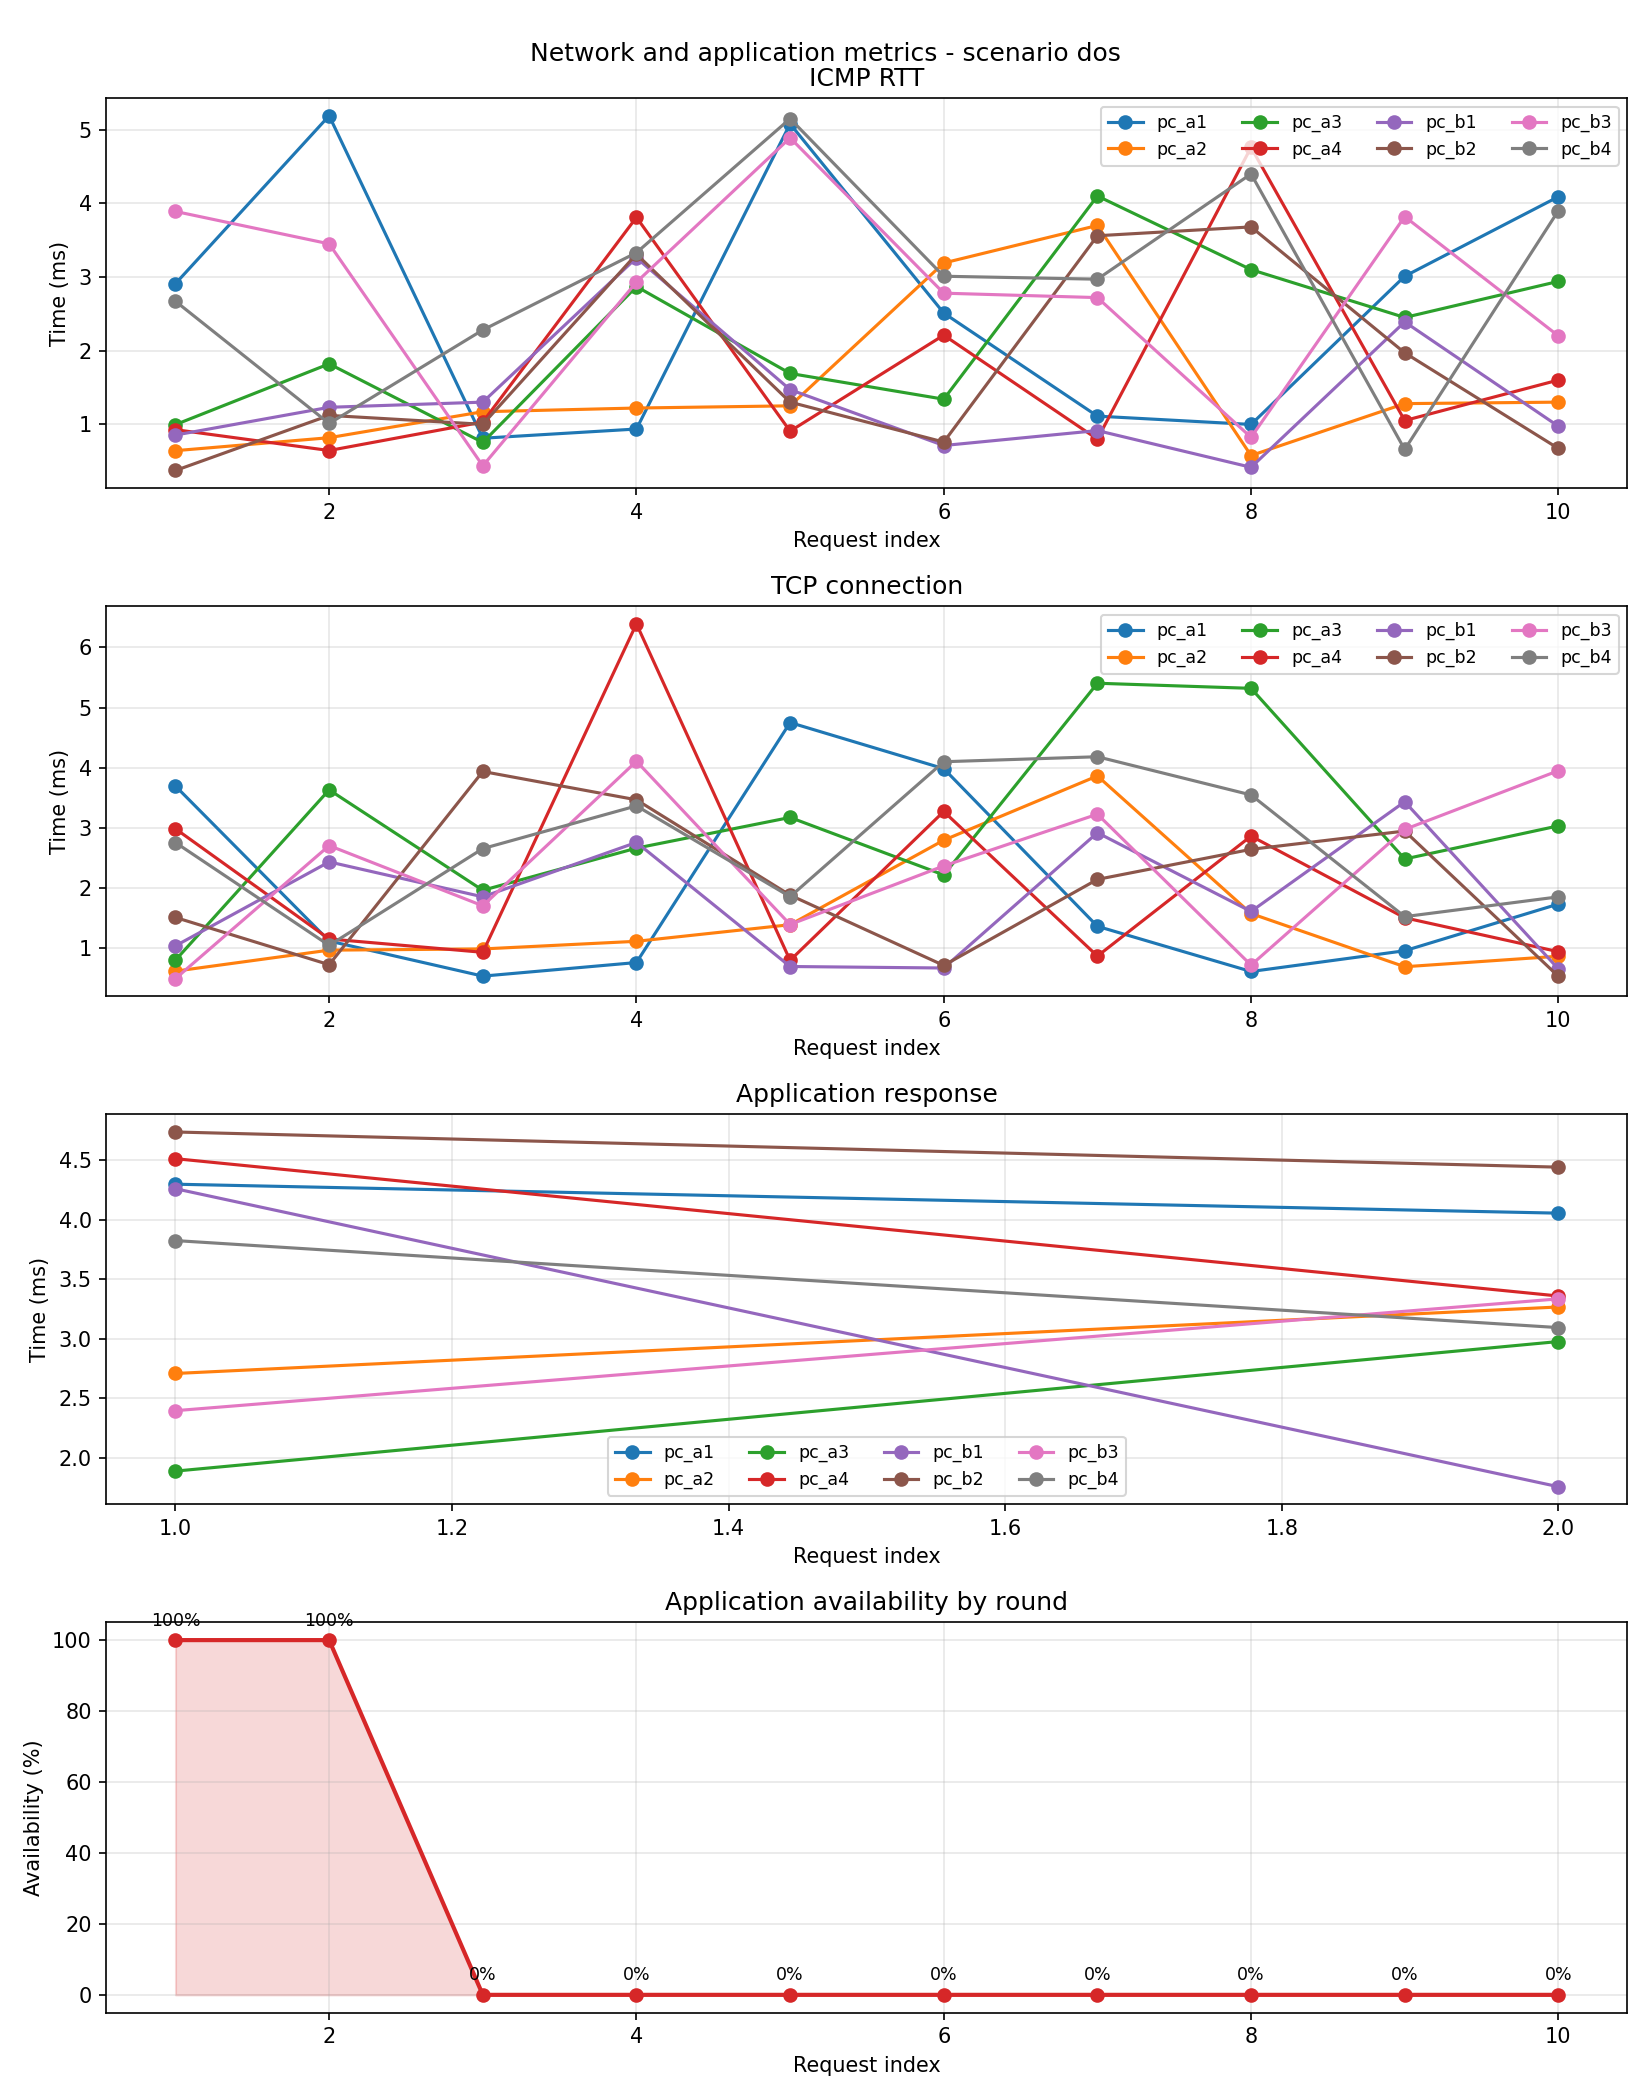
\includegraphics[width=0.90\textwidth]{images/dos_lab_simulation_0001_dos_metrics.png}
\caption{Per-client network and application measurements during the direct-server controlled-load phase in \texttt{dos\_lab/simulation\_0001}.}
\label{fig:direct-dos-metrics}
\end{figure}

Figure~\ref{fig:availability-comparison} separates the complete transition from
the workload-active interval and anticipates the mitigation comparison in
Section~\ref{sec:mitigation-results}. The plot focuses on completed application
requests rather than on ICMP or TCP reachability, because those lower-layer
checks remained successful throughout both experiments.

\begin{figure}[htbp]
\centering
\resizebox{0.98\textwidth}{!}{%
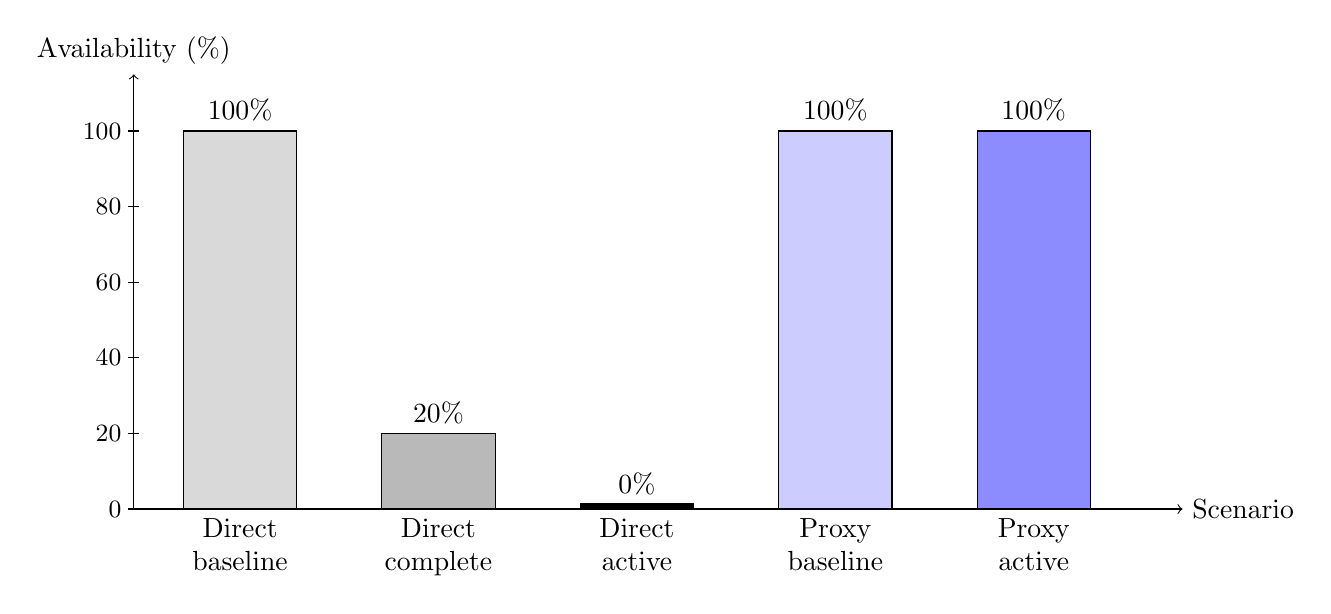
\begin{tikzpicture}[x=0.9cm,y=0.048cm]
    \draw[->] (0,0) -- (14.8,0) node[right] {Scenario};
    \draw[->] (0,0) -- (0,115) node[above] {Availability (\%)};
    \foreach \y in {0,20,40,60,80,100} {
        \draw (-0.08,\y) -- (0.08,\y) node[left=3pt] {\small \y};
    }
    \draw[fill=gray!30] (0.7,0) rectangle (2.3,100);
    \draw[fill=gray!55] (3.5,0) rectangle (5.1,20);
    \draw[line width=2.2pt] (6.3,0.8) -- (7.9,0.8);
    \draw[fill=blue!20] (9.1,0) rectangle (10.7,100);
    \draw[fill=blue!45] (11.9,0) rectangle (13.5,100);
    \node[below,align=center] at (1.5,0) {Direct\\baseline};
    \node[below,align=center] at (4.3,0) {Direct\\complete};
    \node[below,align=center] at (7.1,0) {Direct\\active};
    \node[below,align=center] at (9.9,0) {Proxy\\baseline};
    \node[below,align=center] at (12.7,0) {Proxy\\active};
    \node[above] at (1.5,100) {100\%};
    \node[above] at (4.3,20) {20\%};
    \node[above] at (7.1,1.0) {0\%};
    \node[above] at (9.9,100) {100\%};
    \node[above] at (12.7,100) {100\%};
\end{tikzpicture}
}
\caption{Application availability without and with the reverse-proxy mitigation. ``Complete'' includes the two pre-activation rounds; ``active'' denotes rounds 3--10.}
\label{fig:availability-comparison}
\end{figure}

The service-side counters explain the client observation. During the baseline,
the service recorded 80 accepted connection events and no rejected or
\texttt{BUSY} events. During the controlled-load window it recorded 56 accepted
connection events together with 264 rejected/\texttt{BUSY} events. The maximum
number of simultaneously active application connections reached exactly 20,
which is the configured semaphore limit, and the maximum active thread count
rose from four in the baseline to 25 during the load phase. Periodic server
samples recorded a mean of 15.00 active connections during the
controlled-load scenario, compared with approximately zero at the one-second
sampling instants during the short baseline transactions.

\begin{table}[htbp]
\centering
\small
\begin{tabular}{lrr}
\toprule
\textbf{Server-side observation} & \textbf{Baseline} & \textbf{Controlled load} \\
\midrule
Accepted connection events & 80 & 56 \\
Rejected / \texttt{BUSY} events & 0 & 264 \\
Maximum active connections & 1 & 20 \\
Mean active connections in periodic samples & 0.00 & 15.00 \\
Maximum active threads & 4 & 25 \\
Mean container CPU$^{\dagger}$ & 0.53\% & 2.13\% \\
Maximum container CPU$^{\dagger}$ & 0.88\% & 7.14\% \\
Maximum container memory$^{\dagger}$ & 0.05\% & 0.07\% \\
Maximum container PIDs$^{\dagger}$ & 3 & 23 \\
\bottomrule
\end{tabular}
\caption{Server and container observations for \texttt{dos\_lab/simulation\_0001}. Values marked with $^{\dagger}$ are based on six Docker-stat samples per scenario and are therefore descriptive.}
\label{tab:server-comparison}
\end{table}

The resource samples show higher CPU activity and many more processes/threads
under load, but they should not be over-interpreted. Only six Docker-stat rows
were archived for each scenario, and CPU utilisation on a shared host is
sensitive to scheduling and unrelated host activity. The stronger evidence is
the application-specific instrumentation: the service reached its configured
limit of 20 active connections and generated hundreds of overload rejections
while overall availability fell to 20\% and attack-active availability fell to
0\%. These observations are
directly related by the service implementation and do not depend on a precise
host CPU baseline.

The per-client distribution is also useful. Every legitimate client completed
two out of ten requests, corresponding to 20\% over the complete controlled
run; for every client, both successful requests occurred before workload
activation, so availability during the attack-active interval was 0\%.
There is therefore no indication that a single access LAN or routing path was
responsible for the failures. Instead, the loss of availability appears across
both client networks at the same time, consistent with contention at the common
server endpoint. Combined with the fact that all ICMP probes remained
successful, this supports the interpretation that the routing infrastructure
continued to operate while the application capacity was exhausted.

\section{Reverse-Proxy Mitigation Results}
\label{sec:mitigation-results}

The representative reverse-proxy execution evaluates the mitigation topology
under the same client schedule. A rate-limiting reverse proxy exposes the public endpoint
at \texttt{10.30.1.10:9000} and forwards admitted sessions to a backend at
\texttt{10.30.2.10:9000}. The proxy applies global and per-source connection
limits, while the clients continue to use the same application protocol and
the controlled agents retain the same activation point. Consequently, the
intentional experimental change is the protected service path rather than the
client measurement procedure.

The baseline and controlled-load files in
\path{mitigation/simulation_0002} each contain 80 requests. Every request
succeeded at the ICMP, TCP, and application layers in both phases. In
particular, all 64 legitimate requests in rounds 3--10 completed while the
controlled workload was active, compared with 0 of 64 in the direct-server
experiment. Each of the eight clients therefore achieved ten successes out of
ten, with no difference in availability between the two access LANs.

\begin{table}[htbp]
\centering
\small
\setlength{\tabcolsep}{4pt}
\begin{tabular}{lrrr}
\toprule
\textbf{Client-side metric} & \textbf{Proxy baseline} & \textbf{Proxy load} & \textbf{Direct load} \\
\midrule
Successful application requests & 80 / 80 & 80 / 80 & 16 / 80 \\
Overall application availability & 100.00\% & 100.00\% & 20.00\% \\
Attack-active availability & -- & 100.00\% & 0.00\% \\
Successful ICMP probes & 80 / 80 & 80 / 80 & 80 / 80 \\
Successful TCP handshakes & 80 / 80 & 80 / 80 & 80 / 80 \\
Mean ICMP RTT & 1.550 ms & 1.674 ms & 2.127 ms \\
Mean TCP connection time & 1.808 ms & 1.781 ms & 2.198 ms \\
Mean application response time & 6.058 ms & 5.545 ms & 3.432 ms$^{*}$ \\
Median application response time & 5.896 ms & 5.133 ms & 3.347 ms$^{*}$ \\
95th percentile application response & 9.177 ms & 9.502 ms & 4.567 ms$^{*}$ \\
Maximum application response time & 11.696 ms & 11.019 ms & 4.735 ms$^{*}$ \\
\bottomrule
\end{tabular}
\caption{Client-side results for the mitigation experiment and the corresponding direct-server load phase. Direct-load application latencies marked with $^{*}$ describe only the 16 successful requests.}
\label{tab:mitigation-client-comparison}
\end{table}

Figures~\ref{fig:mitigation-baseline-metrics} and
\ref{fig:mitigation-dos-metrics} show the complete per-client series for the
mitigation experiment. Unlike the direct-server load plot, the application
panel contains observations for every client and round, and the availability
panel remains at 100\% after workload activation.

\begin{figure}[p]
\centering
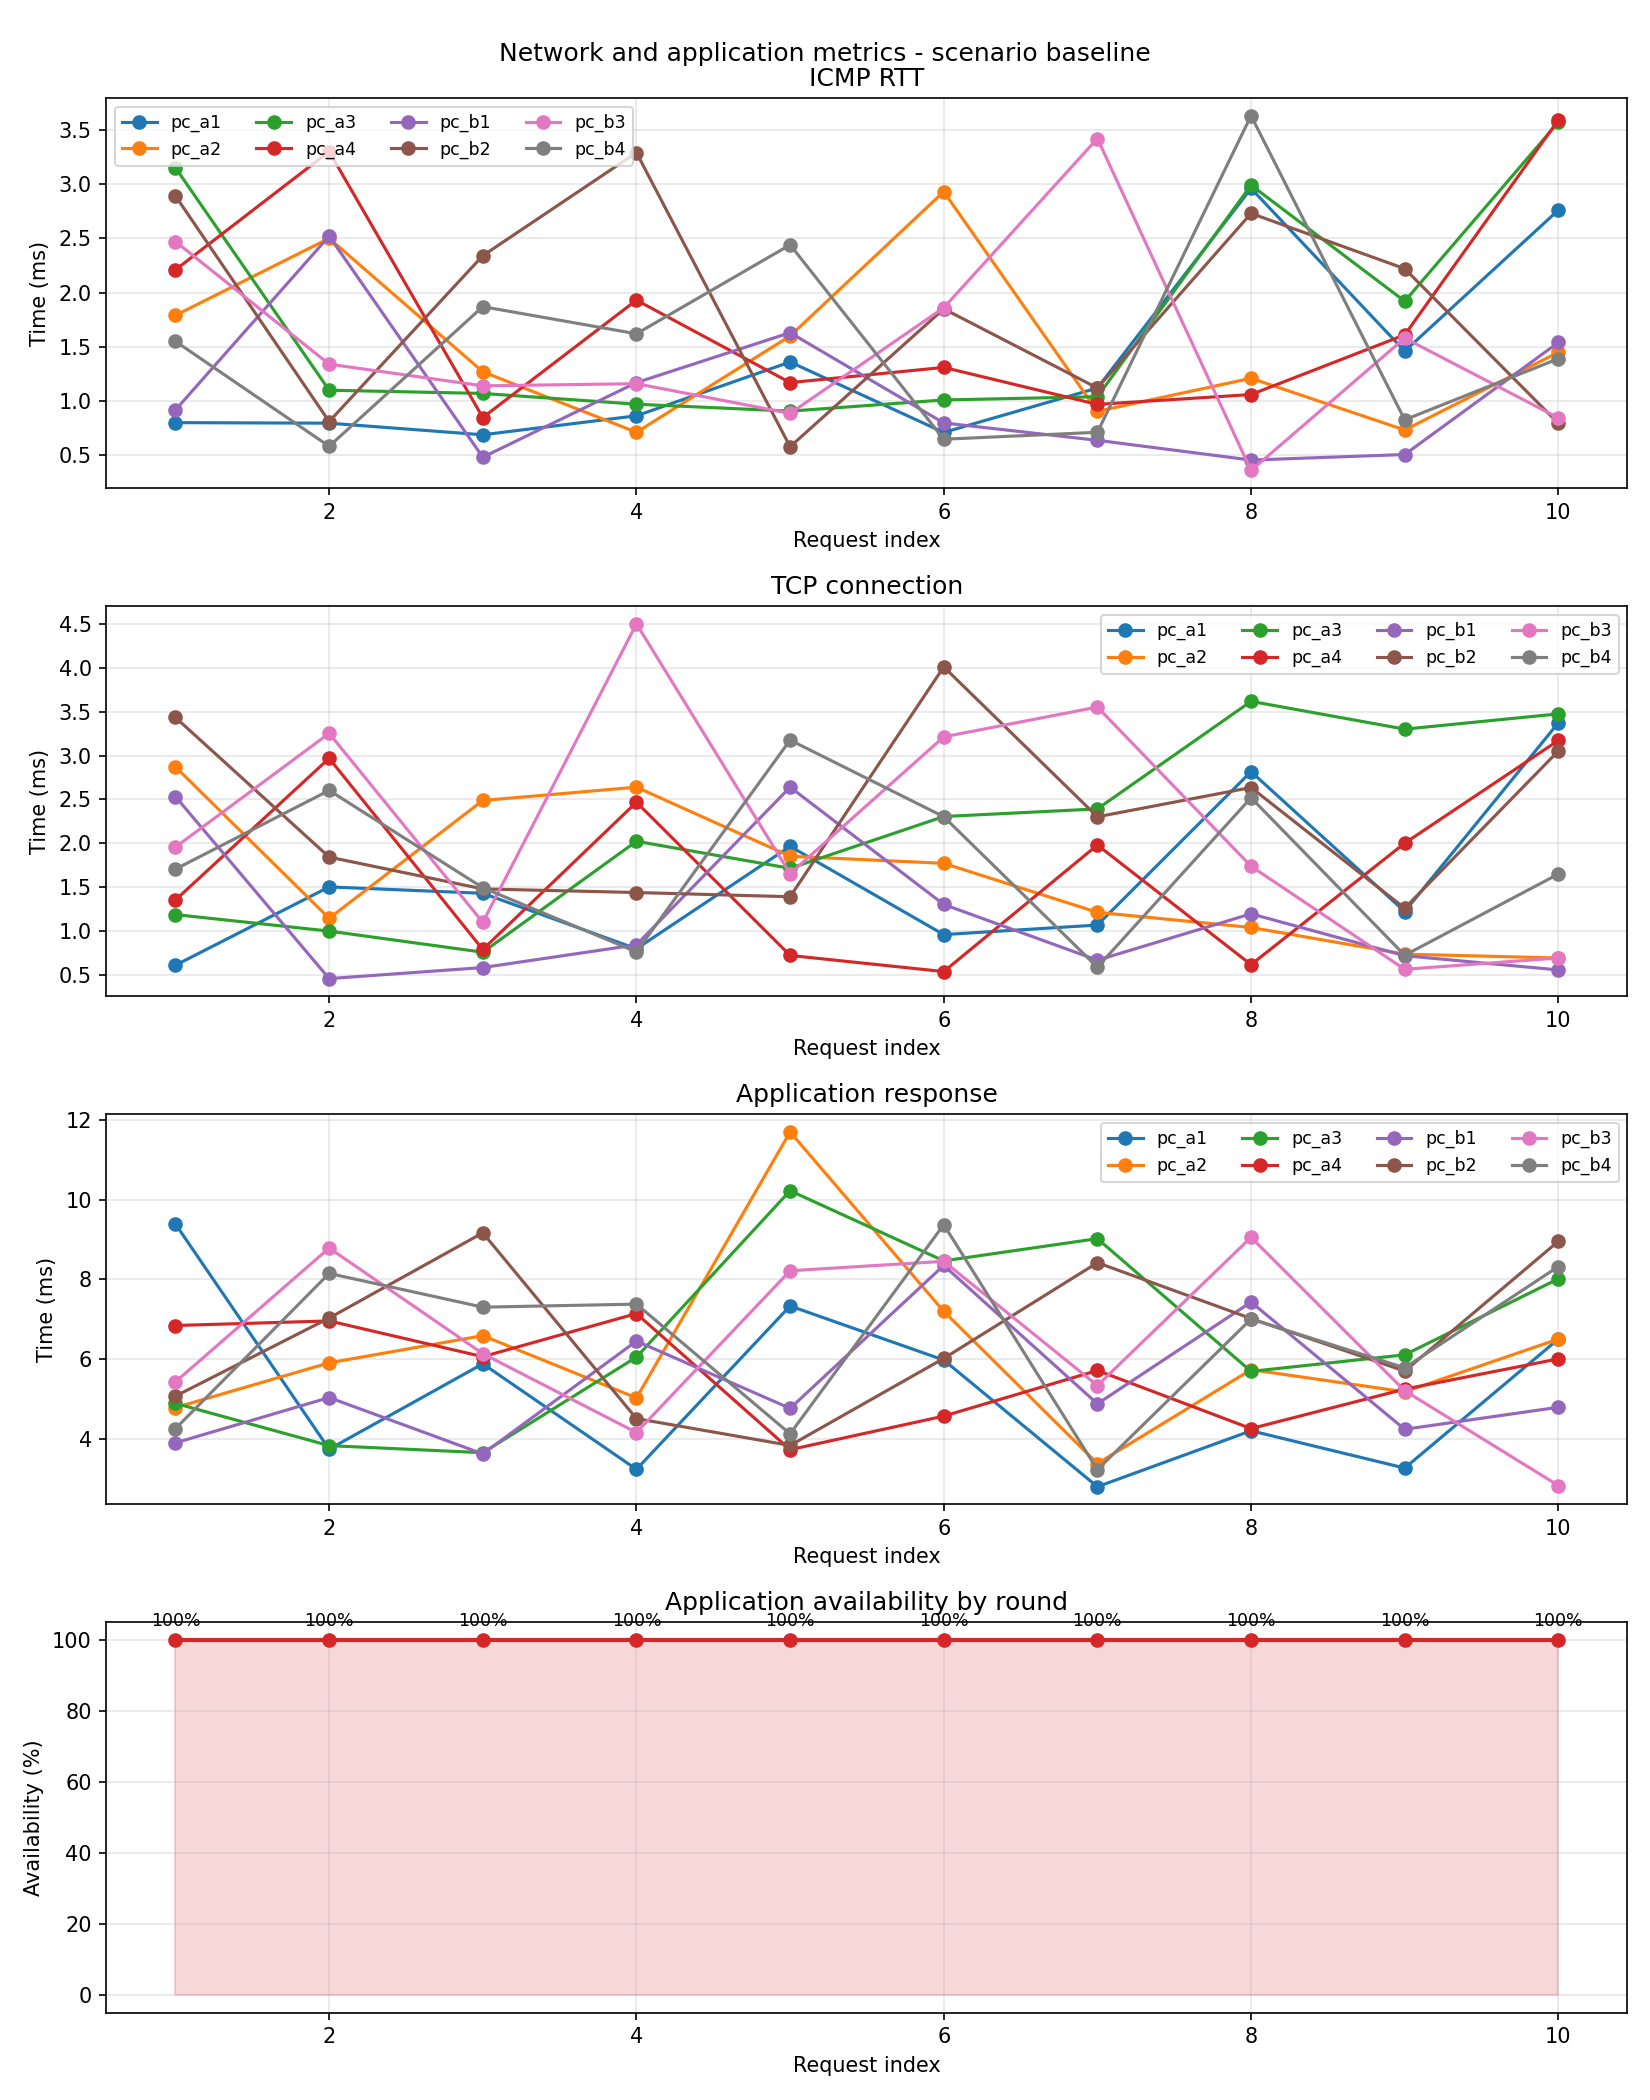
\includegraphics[width=0.90\textwidth]{images/mitigation_simulation_0002_baseline_metrics.png}
\caption{Per-client network and application measurements for the reverse-proxy baseline in \texttt{mitigation/simulation\_0002}.}
\label{fig:mitigation-baseline-metrics}
\end{figure}

\begin{figure}[p]
\centering
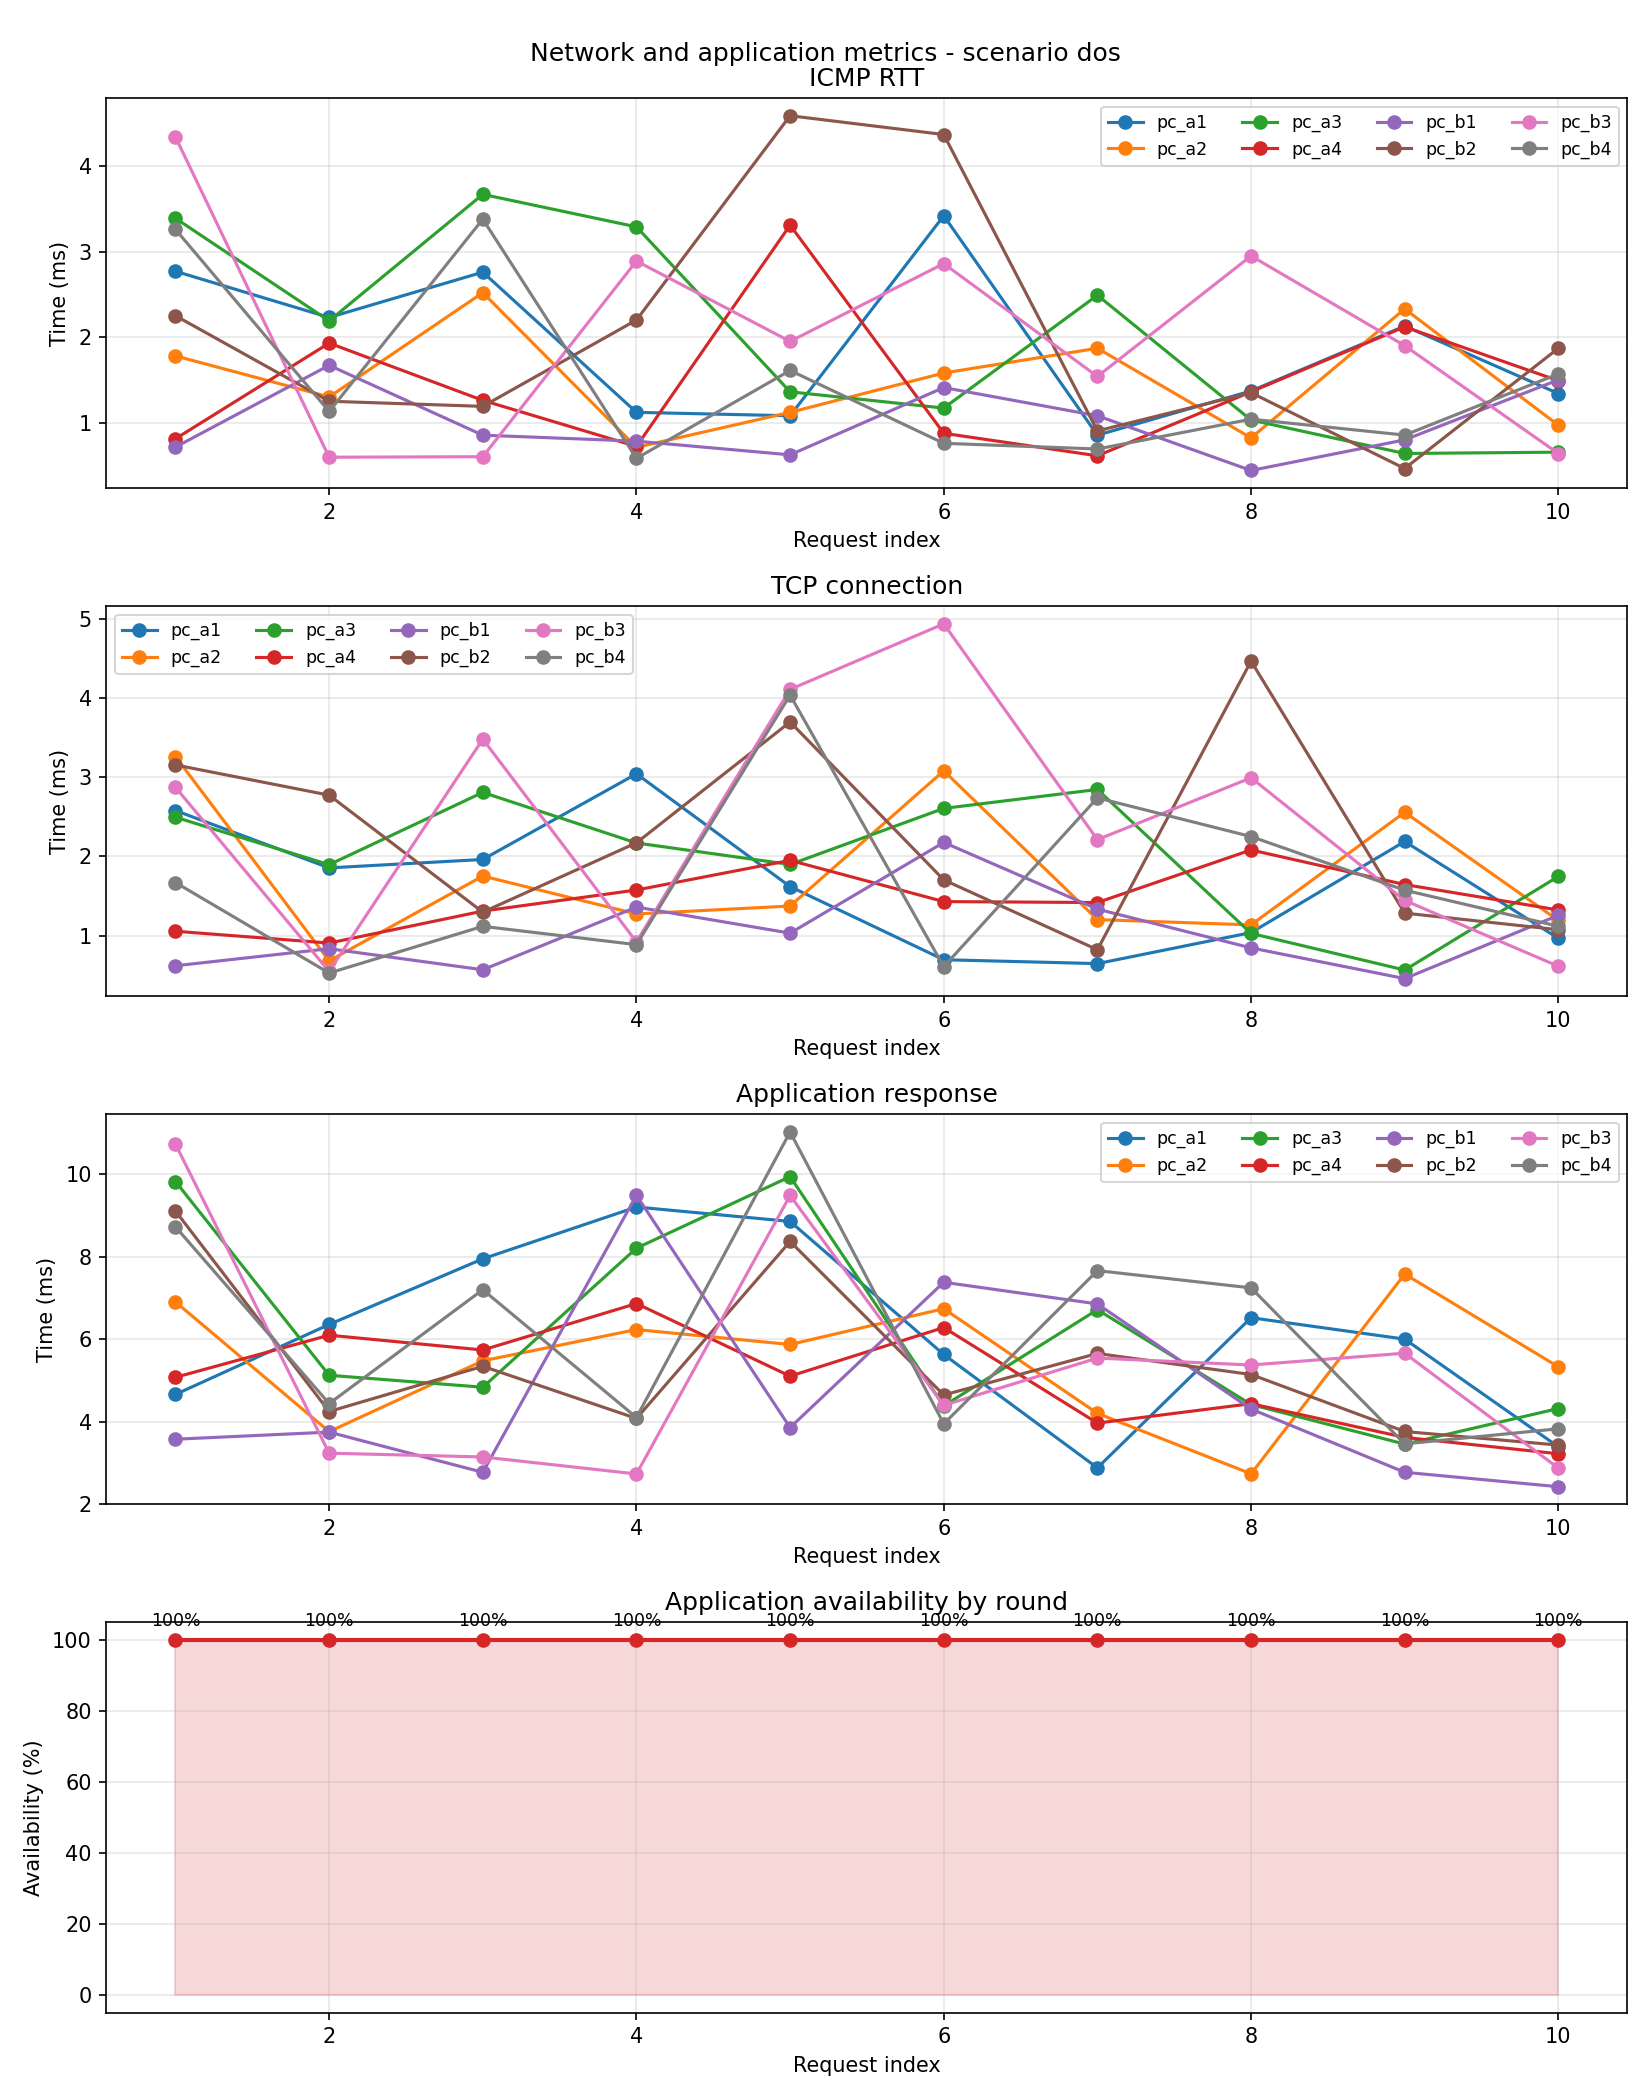
\includegraphics[width=0.90\textwidth]{images/mitigation_simulation_0002_dos_metrics.png}
\caption{Per-client network and application measurements during the reverse-proxy controlled-load phase in \texttt{mitigation/simulation\_0002}.}
\label{fig:mitigation-dos-metrics}
\end{figure}

The proxy introduces a measurable baseline cost: mean application response
time is 6.058 ms through the proxy and 3.218 ms in the direct-server baseline,
a difference of 2.840 ms. This latency difference should be interpreted as a
descriptive observation from one run, not as a stable estimate of proxy
overhead. More importantly for this experiment, the distribution remains
bounded under load: the mitigated mean is 5.545 ms and the 95th percentile is
9.502 ms while all requests complete. The lower mean under load than in the
proxy baseline is another reason not to infer small performance differences
from a single short execution.

The backend instrumentation is consistent with the client-side result. During
the mitigated load phase the backend records 92 accepted connections, no
rejected or \texttt{BUSY} event, and a maximum of eight simultaneous
connections, well below its limit of 20. The count exceeds the 80 legitimate
requests because a limited subset of controlled-workload sessions also reaches
the backend. The reverse proxy therefore does not remove all adverse traffic;
in this run it prevents that traffic from exhausting the backend's application
slots.

\begin{table}[htbp]
\centering
\small
\setlength{\tabcolsep}{4pt}
\begin{tabular}{lrrr}
\toprule
\textbf{Backend observation} & \textbf{Proxy baseline} & \textbf{Proxy load} & \textbf{Direct load} \\
\midrule
Accepted connection events & 80 & 92 & 56 \\
Rejected / \texttt{BUSY} events & 0 & 0 & 264 \\
Maximum active connections & 2 & 8 & 20 \\
Mean active connections in periodic samples & 0.00 & 4.62 & 15.00 \\
Maximum active threads & 4 & 10 & 25 \\
Mean container CPU$^{\dagger}$ & 0.49\% & 0.78\% & 2.13\% \\
Maximum container CPU$^{\dagger}$ & 0.75\% & 1.56\% & 7.14\% \\
Maximum container memory$^{\dagger}$ & 0.05\% & 0.06\% & 0.07\% \\
Maximum container PIDs$^{\dagger}$ & 3 & 9 & 23 \\
\bottomrule
\end{tabular}
\caption{Backend and container observations with mitigation, compared with the unmitigated load phase. Values marked with $^{\dagger}$ are based on six Docker-stat samples per phase.}
\label{tab:mitigation-server-comparison}
\end{table}

These results demonstrate effectiveness only for the bounded,
connection-oriented workload and rate limits used in this laboratory. They do
not establish resistance to volumetric traffic, source-address rotation,
distributed sources that defeat per-source limits, proxy resource exhaustion,
or the application-layer techniques discussed earlier in the chapter. The
representative pair shows that attack-active application availability increases
from 0\% without the proxy to 100\% with it, while the backend maximum falls
from 20 to eight simultaneous connections and overload rejections fall from
264 to zero. Whether these values persist across clean laboratory restarts is
evaluated explicitly in Section~\ref{sec:repeated-run-validation}.

The experiment demonstrates why the measurement framework records several
layers independently. ICMP RTT answers whether the host is reachable; TCP
connection time describes connection establishment; application response time
measures successful transactions; application status captures whether the
transaction actually completed; and server-side counters reveal the internal
capacity state. No single metric is sufficient to describe the experiment. The
combination makes it possible to identify a state in which the network remains
healthy, TCP remains reachable, but the application is no longer reliably
available to legitimate clients.


\section{Repeated-Run Repeatability Analysis}
\label{sec:repeated-run-validation}

To evaluate run-to-run repeatability, the complete baseline and controlled-load
procedure was executed five times for each topology. The runs were organised
as five acquisition blocks, each containing one direct-server run and one
reverse-proxy run; the laboratory was cleaned and restarted between
executions. Client count, round count, timeouts, workload activation point,
number of controlled connection workers, and workload duration were unchanged.
The direct run preceded the mitigated run inside each block, so the pairing
controls the acquisition period but does not remove every possible host-order
effect.

The statistical unit is one complete execution, not one of its 80 client
requests. Request-level observations within a run are dependent because they
share the same emulated network, server process, host scheduler, and workload
episode. Each run was therefore summarised first; descriptive statistics were
then calculated across the five run-level values. Table~\ref{tab:repeated-run-summary}
reports the median, first and third quartiles, and sample variance $s^2$ with
denominator $n-1$. Percentiles within each run use the same nearest-rank method
as \path{show_connection_results.py}. For availability under active load, only
rounds 3--10 are included, yielding 64 legitimate requests per run.

\begin{table}[htbp]
\centering
\small
\setlength{\tabcolsep}{3.5pt}
\begin{tabular}{>{\raggedright\arraybackslash}p{0.32\textwidth}rr@{\hspace{7pt}}rr}
\toprule
& \multicolumn{2}{c}{\textbf{Direct server}} & \multicolumn{2}{c}{\textbf{Reverse proxy}} \\
\cmidrule(lr){2-3}\cmidrule(lr){4-5}
\textbf{Run-level metric} & \textbf{Median [Q1, Q3]} & \boldmath{$s^2$} & \textbf{Median [Q1, Q3]} & \boldmath{$s^2$} \\
\midrule
Baseline availability (\%)
& 100 [100, 100] & 0
& 100 [100, 100] & 0 \\
Active-load availability (\%)
& 0 [0, 0] & 0
& 100 [100, 100] & 0 \\
Baseline application median (ms)
& 3.335 [3.290, 3.336] & 0.088
& 5.808 [5.437, 5.896] & 0.144 \\
Baseline application p95 (ms)
& 5.399 [5.008, 5.900] & 0.338
& 9.514 [9.170, 10.915] & 1.899 \\
Active-load application median (ms)
& -- & --
& 5.315 [5.236, 5.700] & 0.271 \\
Active-load application p95 (ms)
& -- & --
& 9.481 [9.151, 9.540] & 0.663 \\
Rejected / \texttt{BUSY} events
& 264 [264, 264] & 0
& 0 [0, 0] & 0 \\
Maximum active backend connections
& 20 [20, 20] & 0
& 8 [8, 8] & 0 \\
\bottomrule
\end{tabular}
\caption{Run-level descriptive statistics across five complete executions per topology. Variance is the sample variance across runs. Dashes denote an undefined latency statistic because no direct-server request completed during active load.}
\label{tab:repeated-run-summary}
\end{table}

Figure~\ref{fig:repeated-run-comparison} displays the observed run-level values
directly, without fitting a distribution to the five executions. The paired
layout preserves the acquisition-block structure and separates quantities with
different units into distinct panels.

\begin{figure}[p]
    \centering
    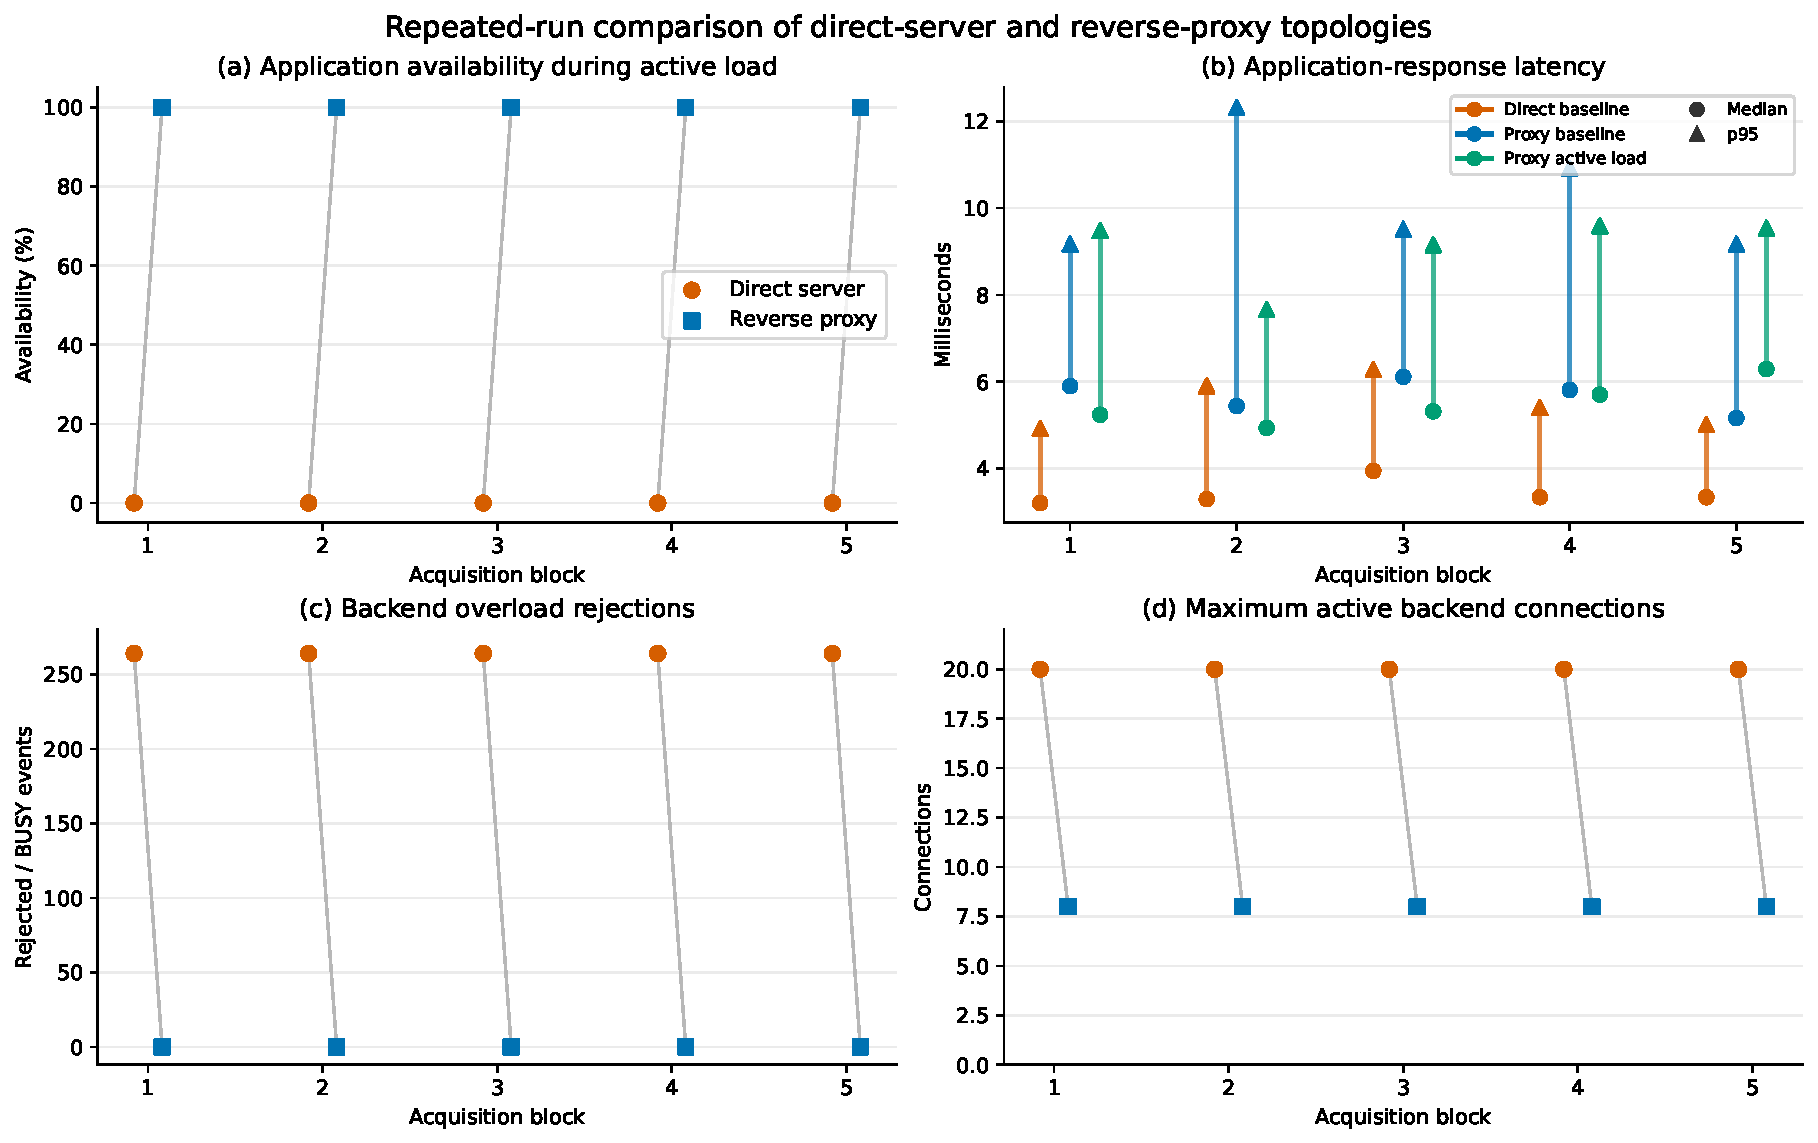
\includegraphics[width=\textwidth]{images/repeated_run_validation.pdf}
    \caption{Run-level comparison across the five paired acquisition blocks.
    Grey lines connect the direct-server and reverse-proxy observations within
    each block. Panel~(a) reports attack-active application availability;
    panel~(b) reports application-response medians and p95 values where a
    transaction completed; panels~(c) and~(d) report backend overload
    rejections and maximum active connections. Direct-server active-load
    latency is absent because no request completed during that interval.}
    \label{fig:repeated-run-comparison}
\end{figure}

All five direct-server baselines and all five reverse-proxy baselines achieved
80 successes out of 80 requests. During the complete transition phase, every
direct-server run achieved 16 successes out of 80, because only the two
pre-activation rounds completed. Consequently, all five direct-server runs had
0 successes out of 64 during active load. In contrast, every reverse-proxy run
completed all 64 active-load requests. The paired availability difference was
therefore $+100$ percentage points in each of the five acquisition blocks:
median $+100$, interquartile interval $[+100,+100]$, and sample variance zero.
This exact replication provides evidence of consistent behaviour for the
tested configuration beyond the original single execution, although five runs
remain a small sample and do not justify extrapolation to other workload
models.

Latency is reported only where an application transaction completed. No
direct-server application latency exists for rounds 3--10, so assigning a
timeout value or comparing the proxy only with the 16 pre-activation direct
successes would bias the result. The protected path instead produced an
active-load median response between 4.934 and 6.288 ms across runs and a p95
between 7.661 and 9.590 ms. In the baseline, the paired increase in the
per-run application median introduced by the proxy had a median of 2.167 ms
and an interquartile interval of [2.147, 2.472] ms. This provides a run-level
estimate of the protection overhead while keeping availability and latency as
separate outcomes.

The server-side evidence is equally stable. Every direct run reached the
20-connection application limit and recorded 264 rejected or \texttt{BUSY}
events during the controlled-load phase. Every mitigated run limited the
backend maximum to eight connections and recorded zero overload rejection.
Thus each paired block reduced the maximum backend occupancy by 12 connections
and the rejection count by 264. The zero variances in these discrete outcomes
describe deterministic repetition under the fixed laboratory parameters; they
must not be interpreted as proof that the same values hold for untested rates,
source populations, protocols, or host environments.

\section{Threats to Validity}
\label{sec:experimental-threats-validity}

The results support a comparison between the two implemented architectures
under the stated parameters, but several threats constrain their
interpretation.

\paragraph{Construct validity.}
Application availability is defined as receipt of the expected response within
the configured timeout. This is stronger than ICMP reachability or completion
of a TCP handshake, but it represents one small TCP service rather than every
notion of service quality. Response time is defined only for completed
transactions; failed requests are therefore reported through availability and
are not assigned an artificial latency. The controlled workload reproduces a
bounded application-layer resource-exhaustion condition generated by known
nodes. It is useful for comparing the direct and protected paths, but it is not
a measurement of Internet-scale DDoS resistance.

\paragraph{Internal validity.}
Both emulated networks, their containers, and the measurement processes share
one physical host. CPU scheduling, filesystem activity, and Docker overhead
can consequently affect clients, workload generators, proxy, and server at the
same time. Pairing the two architectures within acquisition blocks reduces
changes between distant measurement periods, and cleaning and restarting the
laboratory reduces residual runtime state. However, the direct-server run
always preceded the proxy run inside a block, so an order or warm-cache effect
cannot be excluded. The proxy topology also adds both rate limiting and an
extra processing hop; the experiment estimates the effect of the complete
architectural change and does not isolate every proxy mechanism individually.

\paragraph{External validity.}
The experiment uses Kathar\'a and Docker on one workstation, a fixed routed
topology, eight legitimate clients, one application protocol, one server
capacity limit, and one controlled workload profile. Different machines,
container runtimes, network delays, loss patterns, request mixes, proxy rules,
or adversarial strategies may produce different results. In particular, a
distributed workload with many source identities could interact differently
with rate limiting. The observed 0\% and 100\% active-load availability values
therefore characterise the tested configurations and must not be extrapolated
to production services.

\paragraph{Conclusion validity.}
Five paired executions provide stronger evidence than a single demonstration,
and treating each complete run as the statistical unit avoids presenting the
dependent client requests as independent samples. Nevertheless, five pairs are
too few for precise population estimates or a persuasive analysis of small
latency differences. The repeated binary and counter outcomes are reported
descriptively; zero sample variance records what occurred in these runs, not an
absence of variability in the wider population. Further evaluation should
randomise execution order, increase the number of independent restarts, and
vary workload intensity and host conditions before making broader causal or
performance claims.

\section{Chapter Summary}
\label{sec:experimental-summary}

This chapter evaluated the generated framework through a controlled experiment
executed entirely inside Kathar\'a. The testbed combined eight legitimate
clients, an OSPF-based routed core, a separate workload network, and an
instrumented TCP application service. The orchestration layer verified target
reachability before measurement, executed all legitimate clients concurrently
for each round, and stored client, application, server, and container metrics
under a run-specific directory.

Across all five direct-server runs, every baseline produced 80 successful
application transactions out of 80 attempts. Every complete transition run had
20\% availability because its first two rounds preceded workload activation;
during rounds 3--10, every run had 0 successes out of 64 despite successful
ICMP probes and TCP handshakes. In all five executions the service reached its
configured limit of 20 active connections and recorded 264 overload
rejections. The repeated result demonstrates a distinction that is central to
end-to-end service evaluation: network reachability and TCP acceptance do not
necessarily imply application availability.

The five reverse-proxy runs provide the corresponding architectural
comparison. Every baseline and controlled-load phase completed all 80
application requests, including all 64 requests issued during active load. In
each run the protected backend recorded no overload rejection and reached at
most eight simultaneous connections. The paired improvement in active-load
availability was 100 percentage points in every acquisition block, while the
median baseline application-response overhead was 2.167 ms. For the bounded
workload used here, the proxy therefore preserved application availability at
the cost of higher baseline response time. This is repeated evidence for the
tested configuration, not a claim of general DDoS resistance.

The real-world cases discussed at the beginning of the chapter clarify the
scope of this result. Mirai/Dyn provides a structural example of distributed
sources, the GitHub incident illustrates reflection and amplification, HTTP/2
Rapid Reset illustrates application-layer request pressure, and the 2025
Cloudflare case illustrates hyper-volumetric short-duration flooding. The
Kathar\'a experiment does not reproduce those Internet-scale mechanisms.
Rather, it isolates a common availability principle in a controlled setting:
when offered workload exceeds a finite service resource, legitimate
transactions can fail even while lower-layer connectivity remains available.

The results also validate the usefulness of the framework as an experimental
platform. The topology is generated from YAML, the same clients and target can
be reused across scenarios, measurements are executed with a consistent schema,
and runs can be checked using explicit reachability and completion criteria.
Five repeated acquisition blocks show that the principal availability and
backend-capacity outcomes are stable across clean laboratory restarts, while
the reported quartiles and variances make the remaining latency dispersion
explicit.
